\documentclass[11pt]{article}
\usepackage[margin=1in]{geometry}
\usepackage[T1]{fontenc}
\usepackage{lmodern}
\usepackage{microtype}
\usepackage{amsmath,amssymb}
\usepackage{enumitem}
\usepackage{booktabs}
\usepackage{array}
\newcolumntype{L}[1]{>{\raggedright\arraybackslash}p{#1}}
\usepackage{graphicx}
\usepackage[font=small,labelfont=bf]{caption}
\usepackage{tikz}
\usetikzlibrary{arrows.meta,positioning,fit}
\usepackage[colorlinks=true,urlcolor=blue,linkcolor=blue]{hyperref}
\setlist{nosep,leftmargin=*}
\graphicspath{{../figures/}}

\title{How Do Area Chairs Turn Reviews into Decisions?\\[2pt]
\large Exploring the ICLR 2025 Review Data}
\author{CSE 5825 Bayesian Machine Learning --- Project Assignment 1 --- Jiazheng Li}
\date{November 2026}

\begin{document}
\maketitle

\noindent In Project 0, I proposed to predict ICLR 2025 decisions from peer reviews. In this assignment, I narrow the question to one step of the process: \emph{how area chairs (ACs) turn the reviewers' ratings into a decision}. Each paper gets three to five reviews. Each reviewer gives an overall rating from $\{1,3,5,6,8,10\}$, where 5 means ``marginally below the acceptance threshold'' and 6 means ``marginally above''. The AC reads the reviews and the discussion and recommends accept or reject. The usual summary of a paper is its mean rating, but the AC is free to weigh the reviews in other ways. All code is at \url{https://github.com/lijiazheng0917/bml-project}.

\section{Working with data}

\subsection{The data set}

\paragraph{What the data are.} I combine three public releases built from OpenReview (Table~\ref{tab:sources}). All three cover the same 11,672 ICLR 2025 submissions and are joined by the OpenReview paper ID.

\begin{table}[h]
\centering\small
\begin{tabular}{L{3.4cm}L{6.8cm}L{4.2cm}}
\toprule
Source & What I use & How it was collected \\
\midrule
\href{https://github.com/papercopilot/iclr-insights}{ICLR Insights} (Kargaran et al., 2025) & For every reviewer: overall rating, confidence (1--5), and sub-scores for soundness, presentation and contribution (1--4), each \emph{before and after} the rebuttal & Daily snapshots of OpenReview during the review period \\
\href{https://huggingface.co/datasets/demfier/reviewertoo-iclr2025}{ReviewerToo} release & Final decision, primary area, title, abstract, review text, meta-review & Scraped from OpenReview after the decisions \\
\href{https://github.com/papercopilot/paperlists}{Paper Copilot} list & Submission status, including withdrawals & Scraped from OpenReview \\
\bottomrule
\end{tabular}
\caption{Data sources (all CC BY 4.0).}
\label{tab:sources}
\end{table}

\paragraph{How the data were collected.} ICLR runs its review process on OpenReview, where reviews, ratings and decisions are public. OpenReview only shows the latest version of a review, so a rating is lost once the reviewer updates it. The ICLR Insights team saved a snapshot every day during the review period and matched each reviewer across snapshots. This is why we can see each reviewer's rating before and after the rebuttal. They also give a ``tracing score'' that says how sure the match is.

\paragraph{Building the analysis sample.} Table~\ref{tab:sample} shows the steps. ReviewerToo labels withdrawn papers as ``reject'', so I use Paper Copilot to separate them. A paper withdrawn \emph{before} any AC decision (no meta-review) is removed. I keep 109 papers that the AC rejected and the authors withdrew afterwards, and 5 papers withdrawn after acceptance, because the AC did decide them. Finally, I randomly split the papers into a training set (80\%) and a test set (20\%), keeping the mix of decisions the same. \textbf{All figures in this report use only the training set.} The test set stays untouched so that the hypotheses in Section~\ref{sec:hyp} can be tested fairly later.

\begin{table}[h]
\centering\small
\begin{tabular}{lr}
\toprule
Step & Papers \\
\midrule
All submissions & 11,672 \\
\quad removed: withdrawn before a decision & $-$2,874 \\
\quad removed: desk rejected, or conflicting labels & $-$71 \\
Decided by an AC (reject 5,019; poster 3,115; spotlight 380; oral 213) & 8,727 \\
\quad with at least two usable reviewer records (\emph{analysis sample}) & 8,655 \\
\quad\quad training set, 80\% (accept rate 42.5\%) & 6,925 \\
\quad\quad test set, 20\% & 1,730 \\
\bottomrule
\end{tabular}
\caption{From all submissions to the analysis sample.}
\label{tab:sample}
\end{table}

\paragraph{Why the data interest me.} Peer review decides which work gets attention, and many careers depend on it. Yet the last step, where an AC combines several reviews into one decision, is hidden. ICLR is one of the few venues where all reviews, ratings and decisions are public, and the ICLR Insights snapshots even show how each rating changed, so this step can be studied directly. As someone who submits to these conferences, I want to know what actually drives the decision.

\paragraph{Possible biases.}
\begin{enumerate}
\item \textbf{Withdrawn papers are missing.} About a quarter of all submissions were withdrawn before a decision, and not at random: their mean initial rating is 4.0, against 5.0 for decided papers, and more than half of the papers with an initial mean below 4 were withdrawn. The results describe papers whose authors chose to stay in the process.
\item \textbf{One conference, one year.} The rating scale, reviewers and AC guidelines are specific to ICLR 2025.
\item \textbf{Reviewers are not assigned at random.} Reviewers bid on papers and are matched by expertise, so ratings and confidence partly reflect who chose to review a paper.
\item \textbf{The AC sees more than we do.} ACs read the paper and the full discussion. If, for example, a low rating points to a real flaw that the AC also sees, this information is missing from our data and can explain part of any pattern we find.
\item \textbf{Rating histories are reconstructed.} For 1,379 papers in the analysis sample (16\%), the tracing score is 2 or more, so the before/after match may be wrong.
\item \textbf{Discussion text is incomplete.} The text release keeps only top-level posts; the authors' replies under each review are missing. This assignment uses only ratings, but it limits later text analysis.
\item \textbf{Authors may not be anonymous.} Many papers are on arXiv, so some reviewers may know who wrote them. We cannot observe this.
\end{enumerate}

\subsection{Three visualizations}

Each figure looks at one way in which ACs might combine ratings. The figures describe patterns in the training set; they are not tests.

\begin{figure}[p]
\centering
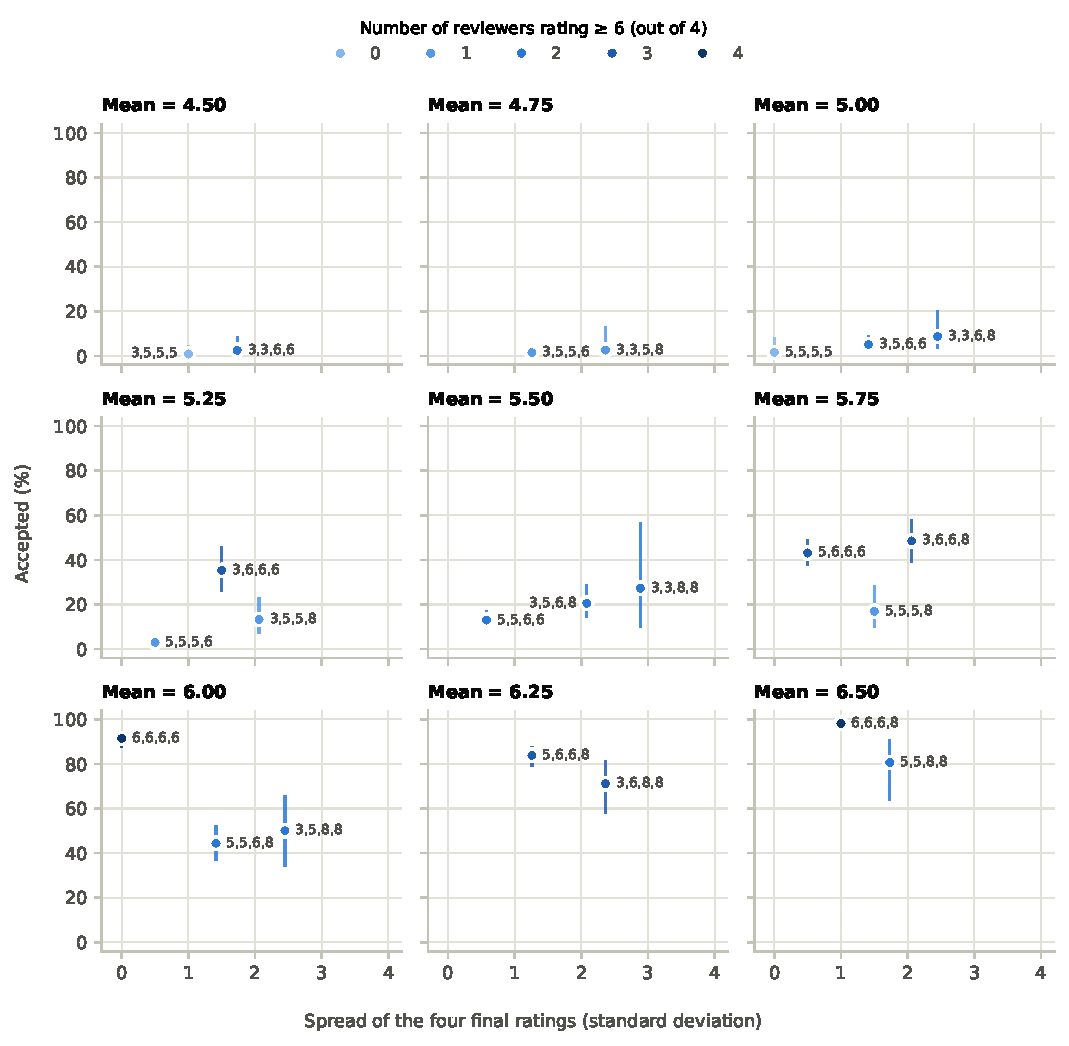
\includegraphics[width=\textwidth]{fig1_spread.pdf}
\caption{Acceptance rate for each combination of four final ratings, with one panel per mean rating (training set, papers with exactly four reviewers, $n=4{,}656$). Each dot is one combination seen in at least 10 papers; the vertical line is a 95\% confidence interval. The x-axis is the spread (standard deviation) of the four ratings. Darker dots have more reviewers on the accept side (rating $\ge 6$).}
\label{fig:spread}
\end{figure}

\paragraph{Figure~\ref{fig:spread}: same mean, different ratings.}
\emph{What it shows.} If ACs used only the mean rating, all dots in a panel would sit at the same height. They do not. Within each panel, the dots are ordered by colour, not by spread: the more reviewers give 6 or higher, the higher the acceptance rate. At a mean of 5.25, papers rated 3,6,6,6 were accepted 35\% of the time, but papers rated 5,5,5,6 only 3\%. At a mean of 6.0, papers rated 6,6,6,6 were accepted 91\% of the time, but 5,5,6,8 only 44\%.
\emph{Why it is interesting.} A single low rating does not sink a paper: 3,6,6,6 does far better than 5,5,5,6, although it contains the lowest rating. This goes against my starting idea that one strong negative review works as a veto. It suggests that ACs count recommendations (accept side vs.\ reject side) instead of averaging numbers. The only hint in the other direction is at a mean of 6.25, where 3,6,8,8 (71\%) is below 5,6,6,8 (84\%), but the two intervals overlap.
\emph{What it tells us about the data.} In practice the rating scale does not behave like evenly spaced numbers: the step from 5 to 6 seems to matter much more than its size of one point.

\begin{figure}[t]
\centering
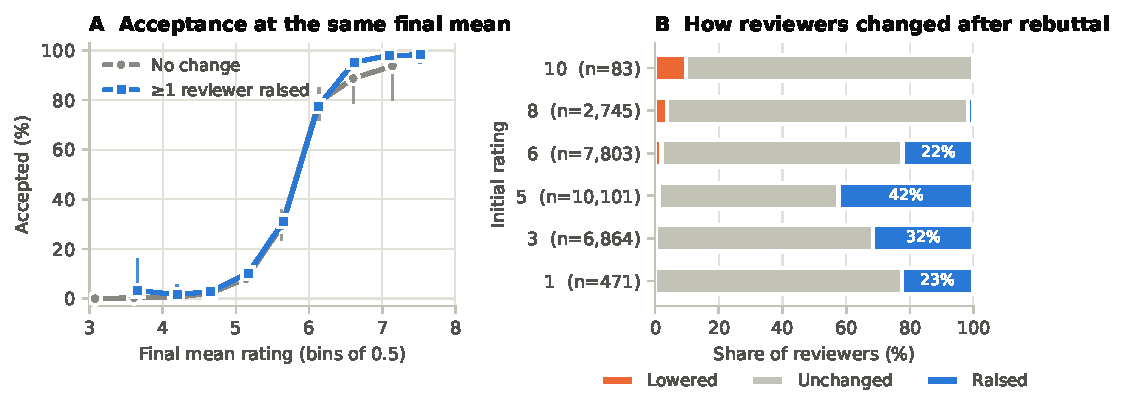
\includegraphics[width=\textwidth]{fig2_raised.pdf}
\caption{(A) Acceptance rate against the final mean rating, for papers where at least one reviewer raised the rating after the rebuttal (and nobody lowered it), and for papers where no rating changed. Final means are grouped in bins of 0.5; vertical lines are 95\% confidence intervals. (B) How reviewers changed their rating after the rebuttal, by their initial rating. Training set.}
\label{fig:raised}
\end{figure}

\paragraph{Figure~\ref{fig:raised}: what the rebuttal changes.}
\emph{What it shows.} Rebuttals move ratings almost only upward: 29.7\% of reviewers raised their rating, 1.5\% lowered it, and 68.8\% kept it (panel B). The most common change is 5$\to$6 (3,904 reviewers), which is exactly the move from ``below the threshold'' to ``above the threshold''. Next come 6$\to$8 (1,732) and 3$\to$5 (1,422). Reviewers who started at 5 changed most often (42\% raised). In panel A, the two curves lie on top of each other: at the same final mean, papers that got there through a rebuttal increase are accepted about as often as papers that had that mean from the start.
\emph{Why it is interesting.} Panel A suggests that ACs mostly look at where the ratings ended, not how they got there. But Figure~\ref{fig:spread} says that ACs care about the \emph{number} of accept-side ratings, and panel B shows that rebuttals mostly create new accept-side ratings (5$\to$6). The figure cannot tell whether such a converted rating counts as much as one that was on the accept side from the start. To see that, we must also hold the number of accept-side ratings fixed, which needs the model in Section~\ref{sec:models}.

\begin{figure}[t]
\centering
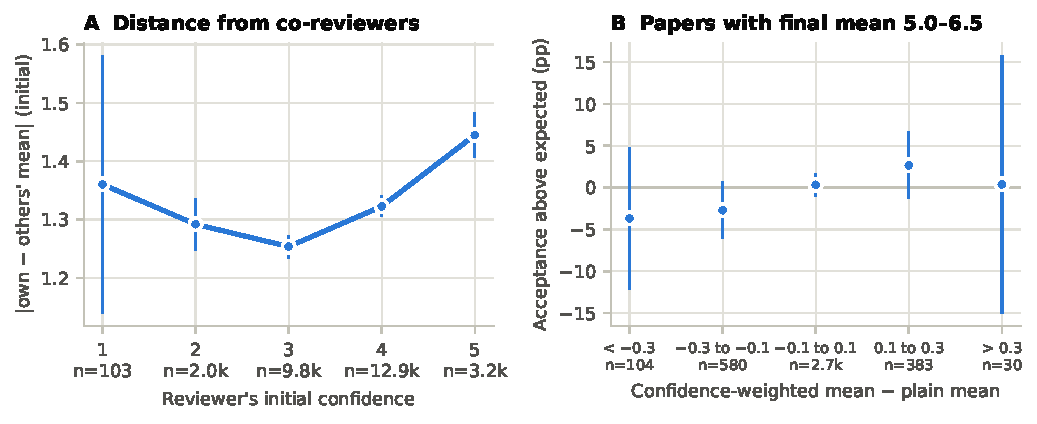
\includegraphics[width=\textwidth]{fig3_confidence.pdf}
\caption{(A) Average distance between a reviewer's initial rating and the mean initial rating of the \emph{other} reviewers of the same paper, by the reviewer's confidence. (B) Papers with a final mean between 5.0 and 6.5: actual acceptance rate minus the rate expected from the mean alone (the acceptance rate of all training papers with exactly the same mean), grouped by how much the confidence-weighted mean differs from the plain mean. Positive x-values mean that the more confident reviewers liked the paper more. Error bars are 95\% confidence intervals.}
\label{fig:confidence}
\end{figure}

\paragraph{Figure~\ref{fig:confidence}: how confidence is used.}
\emph{What it shows.} Panel A: a reviewer's confidence says little about how close the reviewer is to the other reviewers. The distance is smallest at confidence 3 (1.25 points) and largest at confidence 5 (1.45 points). If high confidence meant high accuracy, the line would go down; instead it is U-shaped. Panel B: when the confident reviewers are more negative than the others, papers are accepted about 3--4 percentage points less often than their mean predicts; when the confident reviewers are more positive (0.1 to 0.3), about 3 points more often. The 30 papers above 0.3 give no clear signal.
\emph{Why it is interesting.} Together, the panels suggest that ACs listen more to confident reviewers, even though confidence does not mark the reviewers who agree with their peers. This would be a mismatch between how ACs use confidence and how informative it is. The effect is small and most papers sit in the middle bin, so it needs careful testing.

\section{Thinking about models}
\label{sec:models}

\subsection{Observed variables and their relationships}

Table~\ref{tab:vars} lists the observed variables for paper $i$ and reviewer $j$. From them I compute the final mean rating $\bar r^{(1)}_i$ and the number of accept-side ratings $V_i=\#\{j: r^{(1)}_{ij}\ge 6\}$.

\begin{table}[h]
\centering\small
\begin{tabular}{lll}
\toprule
Symbol & Meaning & Values \\
\midrule
$r^{(0)}_{ij},\ r^{(1)}_{ij}$ & overall rating before / after the rebuttal & $\{1,3,5,6,8,10\}$ \\
$c^{(0)}_{ij},\ c^{(1)}_{ij}$ & reviewer confidence before / after & 1--5 \\
$s^{(0)}_{ijk},\ s^{(1)}_{ijk}$ & sub-score $k$ (soundness, presentation, contribution) & 1--4 \\
$J_i$ & number of reviewers & mostly 3--5 \\
$a_i$ & primary research area & 21 areas \\
$Y_i$ & decision & reject, poster, spotlight, oral \\
\bottomrule
\end{tabular}
\caption{Observed variables.}
\label{tab:vars}
\end{table}

\paragraph{Expected relationships.}
\begin{itemize}
\item \textbf{Ratings and sub-scores move together.} The overall rating is most related to contribution (rank correlation 0.65), then soundness (0.59), then presentation (0.46).
\item \textbf{Confidence is almost unrelated to the rating}; confident reviewers give slightly lower ratings (rank correlation $-0.14$).
\item \textbf{Initial and final ratings are strongly related}: 69\% of reviewers keep their rating.
\item \textbf{The decision depends strongly on the final ratings} (Figure~\ref{fig:spread}). The acceptance rate is a bit lower for papers with more reviewers (47\% with three, 42\% with four, 41\% with five), possibly because extra reviewers are added to difficult papers.
\end{itemize}

\paragraph{Independence and conditional independence.}
\begin{itemize}
\item \textbf{Different papers} are treated as independent given the shared parameters. This is not exactly true (a reviewer or an AC handles several papers), but reviewer and AC IDs are not linked across papers, so we cannot model it.
\item \textbf{Initial ratings of the same paper} are correlated, because they respond to the same paper. But reviewers write their first reviews without seeing each other's, so I expect them to be \emph{independent given the paper's hidden quality} $q_i$: $r^{(0)}_{ij}\perp r^{(0)}_{ij'}\mid q_i$. The correlation is weak: only 15\% of the variation in initial ratings is between papers (intraclass correlation, ICC $=0.15$); the rest is disagreement among reviewers of the same paper.
\item \textbf{Final ratings are not independent given quality}, because reviewers read each other's reviews and the discussion before updating. The data agree: the ICC rises from 0.15 to 0.33 after the rebuttal, so reviewers move toward each other.
\item \textbf{The decision.} Each hypothesis in Section~\ref{sec:hyp} claims that one conditional independence \emph{fails}: H1, $Y_i\perp V_i\mid \bar r^{(1)}_i$ (votes matter beyond the mean); H2, $Y_i\perp r^{(0)}_{i\cdot}\mid r^{(1)}_{i\cdot}$ (initial ratings matter beyond the final ones); H3, $Y_i\perp c_{i\cdot}\mid r^{(1)}_{i\cdot}$ (confidence matters beyond the ratings).
\end{itemize}

\subsection{Hidden variables}

Several important quantities are not observed. Figure~\ref{fig:model} shows how they connect to the data.

\begin{itemize}
\item $q_i$ --- \textbf{paper quality}: what all reviewers try to judge. It explains why ratings of the same paper are correlated, and why initial ratings are independent once we know it.
\item $u^{(0)}_{ij}, u^{(1)}_{ij}$ --- \textbf{a reviewer's opinion on a continuous scale}, before and after the rebuttal. The rating is this opinion cut into six bins, and the cut points are learned, so the model does not assume that the step from 5 to 6 is worth exactly one point. It also explains why an opinion can change while the rating stays the same.
\item $\tau_{ij}$ --- \textbf{reviewer precision}: how close the reviewer's opinion is to the paper's quality. The reported confidence is the reviewer's own guess of $\tau_{ij}$, and the model lets us check how good that guess is.
\item $\rho_i$ --- \textbf{rebuttal effect}: how much the authors' response moves all reviewers of the paper. Reviewers moving toward each other is a second, within-paper effect that is not drawn in Figure~\ref{fig:model}.
\item $t_a$ --- \textbf{acceptance threshold of research area $a$}, with a shared prior so that small areas borrow information from large ones.
\item $\eta_i$ --- \textbf{AC private information}: what the AC learns from the paper and the discussion beyond the ratings. We cannot measure it, so the model treats it as random noise with a fixed scale, and all other effects are measured relative to it.
\end{itemize}

\begin{figure}[t]
\centering
% Graphical model for Section 2.2 (included by proj1_report.tex)
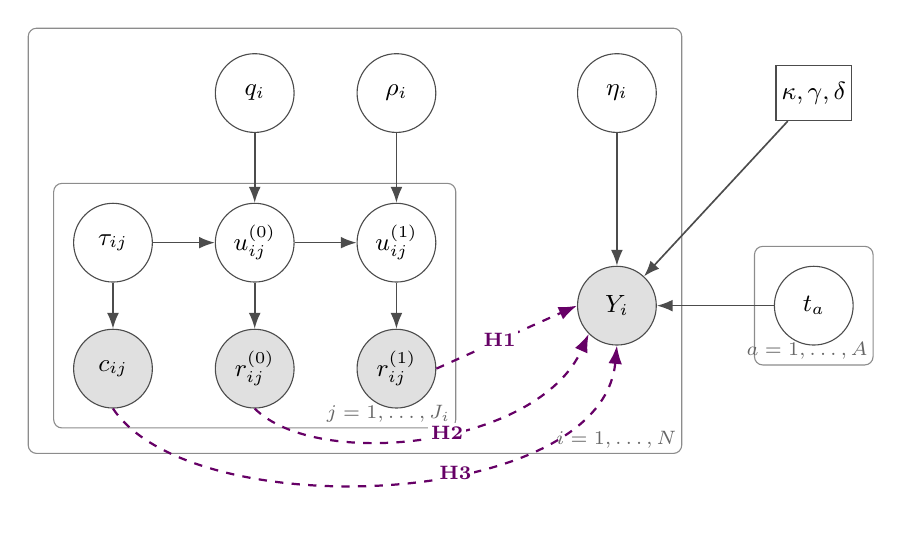
\begin{tikzpicture}[
  >=Latex,
  latent/.style={circle,draw=black!70,minimum size=10mm,inner sep=0pt,font=\small},
  obs/.style={latent,fill=black!12},
  param/.style={rectangle,draw=black!70,fill=white,minimum size=7mm,inner sep=2pt,font=\small},
  arr/.style={->,semithick,draw=black!70},
  test/.style={->,thick,draw=violet!80!black,dashed},
  hyp/.style={font=\scriptsize\bfseries,text=violet!80!black,fill=white,inner sep=1pt},
  platebox/.style={draw=black!45,rounded corners=3pt,inner sep=7pt},
  platelabel/.style={font=\scriptsize,text=black!60,anchor=south east,inner sep=2pt}
]
  % reviewer-level
  \node[latent] (tau) at (0,0)      {$\tau_{ij}$};
  \node[obs]    (c)   at (0,-1.6)   {$c_{ij}$};
  \node[latent] (u0)  at (1.8,0)    {$u^{(0)}_{ij}$};
  \node[obs]    (r0)  at (1.8,-1.6) {$r^{(0)}_{ij}$};
  \node[latent] (u1)  at (3.6,0)    {$u^{(1)}_{ij}$};
  \node[obs]    (r1)  at (3.6,-1.6) {$r^{(1)}_{ij}$};
  \node[platebox, fit=(tau)(c)(u0)(r0)(u1)(r1)] (pj) {};
  \node[platelabel] at (pj.south east) {$j=1,\dots,J_i$};

  % paper-level
  \node[latent] (q)   at (1.8,1.9)  {$q_i$};
  \node[latent] (rho) at (3.6,1.9)  {$\rho_i$};
  \node[latent] (eta) at (6.4,1.9)  {$\eta_i$};
  \node[obs]    (y)   at (6.4,-0.8) {$Y_i$};
  \node[platebox, fit=(pj)(q)(rho)(eta)(y), inner sep=9pt] (pi) {};
  \node[platelabel] at (pi.south east) {$i=1,\dots,N$};

  % global and area-level
  \node[latent] (t)   at (8.9,-0.8) {$t_a$};
  \node[platebox, fit=(t)] (pa) {};
  \node[platelabel] at (pa.south east) {$a=1,\dots,A$};
  \node[param]  (ac)  at (8.9,1.9)  {$\kappa,\gamma,\delta$};

  % edges
  \draw[arr] (tau) -- (c);
  \draw[arr] (tau) -- (u0);
  \draw[arr] (q) -- (u0);
  \draw[arr] (u0) -- (r0);
  \draw[arr] (u0) -- (u1);
  \draw[arr] (rho) -- (u1);
  \draw[arr] (u1) -- (r1);
  \draw[arr] (eta) -- (y);
  \draw[arr] (t) -- (y);
  \draw[arr] (ac) -- (y);

  % edges whose form or existence the hypotheses test
  \draw[test] (r1.east) -- node[hyp,pos=0.45] {H1} (y.west);
  \draw[test] (r0.south) .. controls (2.6,-2.9) and (5.4,-2.6) .. node[hyp,pos=0.55] {H2} (y.south west);
  \draw[test] (c.south) .. controls (1.0,-3.6) and (6.2,-3.4) .. node[hyp,pos=0.6] {H3} (y.south);
\end{tikzpicture}

\caption{Graphical model. Grey circles are observed, white circles are hidden, and the square box holds the shared parameters of the AC rule. Rounded rectangles are plates (repeated for each reviewer, paper and area). Dashed purple arrows are the links that the three hypotheses are about.}
\label{fig:model}
\end{figure}

\paragraph{The AC's rule.} On top of these, I model the decision as
\[
\Pr(Y_i=\text{accept}) = \operatorname{logistic}\bigl(S_i - t_{a(i)}\bigr),\qquad
S_i=\sum_{j} w_{ij}\Bigl[(1-\delta)\,v\bigl(r^{(1)}_{ij}\bigr)+\delta\, v\bigl(r^{(0)}_{ij}\bigr)\Bigr],\qquad
w_{ij}\propto e^{\gamma\, c^{(1)}_{ij}},
\]
where the weights $w_{ij}$ of a paper sum to one and the logistic noise is the AC's private information $\eta_i$. Three shared parameters describe the AC:
$v(k)$ is the value the AC gives to a rating of $k$ (one free number per rating level);
$\delta$ is the weight on the \emph{initial} ratings;
$\gamma$ says how much more the AC listens to confident reviewers.
If $v(k)$ is a straight line in $k$, $\delta=0$ and $\gamma=0$, the rule is simply ``use the mean final rating''. Spotlight and oral can be added later as higher thresholds on the same score.

To ask whether the AC's rule is \emph{reasonable}, I also fit a measurement model to the initial ratings: $u^{(0)}_{ij}=q_i+\varepsilon_{ij}$ with $\varepsilon_{ij}\sim\mathcal N(0,\sigma^2(c_{ij}))$, and $r^{(0)}_{ij}$ is $u^{(0)}_{ij}$ cut into bins. Because initial ratings are independent given $q_i$, their agreement tells us how much each rating level and each confidence level says about quality. From this we can work out how an \emph{ideal AC} --- one that ranks papers by their expected quality given all ratings --- would weigh the ratings, and compare it with the fitted $v$, $\delta$ and $\gamma$.

\subsection{Hypotheses}
\label{sec:hyp}

Each hypothesis has two parts: (a) a \textbf{pattern} that should also appear in the held-out test set, and (b) a \textbf{deeper question}: does the AC behave like the ideal AC above? Part (b) cannot be read off a figure; it needs the hidden-variable model.

\paragraph{H1: ACs count votes.}
(a) At the same final mean rating, the chance of acceptance rises with the number of reviewers who rate the paper 6 or higher; a single low rating ($\le 3$) does not work as a veto.
(b) In the AC rule, the gap $v(6)-v(5)$ is larger than the gaps $v(5)-v(3)$ and $v(8)-v(6)$, and larger than an ideal AC would use. In plain words: ACs treat a rating mainly as an accept/reject recommendation.
\emph{Why I expect it:} Figure~\ref{fig:spread}, and the rating labels themselves (``marginally below/above the threshold'') read like votes.
\emph{What would count against it:} adding the vote count, or free values $v(k)$, does not improve predictions on the test set; or the fitted $v(k)$ lie close to a straight line.

\paragraph{H2: converted votes count less.}
(a) Among papers with the same final mean and the same number of accept-side ratings, papers in which a reviewer moved from below 6 to 6 or higher during the rebuttal are accepted less often than papers whose accept-side ratings were there from the start.
(b) $\delta>0$: the AC keeps some weight on the initial ratings. An ideal AC should do this, because initial ratings are independent opinions, while final ratings partly reflect reviewers moving toward each other (ICC 0.15 $\to$ 0.33).
\emph{Why I expect it:} 5$\to$6 is the most common change (Figure~\ref{fig:raised}B), and ACs can see the rating history and the discussion.
\emph{What would count against it:} $\delta$ close to 0 (ACs use only the final ratings, as Figure~\ref{fig:raised}A suggests at the level of the mean), or $\delta<0$ (ACs reward a successful rebuttal).

\paragraph{H3: confidence gets too much weight.}
(a) At the same final mean and number of accept-side ratings, papers whose confident reviewers are more positive than their less confident reviewers are accepted more often ($\gamma>0$).
(b) In the measurement model, a reviewer's noise $\sigma(c)$ hardly shrinks with confidence, so the AC's weight on confidence is larger than an ideal AC would use.
\emph{Why I expect it:} Figure~\ref{fig:confidence}B for part (a) and Figure~\ref{fig:confidence}A for part (b).
\emph{What would count against it:} $\gamma$ close to 0; or $\sigma(c)$ clearly shrinks with confidence, in which case listening to confident reviewers is reasonable.

\paragraph{How I will test them (Projects 2--3).}
\begin{enumerate}
\item The hypotheses and the analysis plan are fixed now, before anyone looks at the test set.
\item Fit the AC rule and the measurement model with MCMC on the training set, and report posterior intervals for $v(k)$, $\delta$, $\gamma$ and $\sigma(c)$.
\item Compare versions of the AC rule (mean only; mean plus vote count; free $v(k)$; with and without $\delta$ and $\gamma$) by their log-likelihood on the 20\% test set.
\item Posterior predictive check: simulate decisions from the fitted model and check that they reproduce Figure~\ref{fig:spread}.
\item Repeat the analysis on ICLR 2024, which ICLR Insights also covers with the same rating scale.
\item Check sensitivity: use only reviewers with a tracing score of 1 or less, and treat the rejected-then-withdrawn papers differently.
\end{enumerate}

\end{document}
